\part{Algebraic Geometry, Hartshorne}
In this part, I will be going through the work of Hartshorne as he laid out in \cite{hartshorne2013algebraic}. The book is sectioned into 5 distinct chapters - 'Varieties', 'Schemes', 'Cohomology', 'Curves' and 'Surfaces'. We study them in order as they flow nicely. 

\section{Varieties}

\begin{definition}
\textbf{Affine $n$-Space over $k$: } Let $k$ be a field and $n \in \N$. Then the affine $n$-space over $k$ is defined
\[\Aff_k^n = \{(k_1,...,k_n)\in k^n\}\]
\end{definition}
It seems that this is a silly definition, but later on we will see that it is useful to have a distinction between the variety $\Aff^n_k$ and the set of points in $k^n$. We later view $\Aff_k^n$ as an affine variety - an object in some arbitrary space rather than the set of $k$-tuples. 

Let $A = k[x_1,...,x_n]$ be the polynomial ring over $k$ in $n$ variables. Then $f\in A$ is a map $f: k^n \to k$. We define the vanishing locus of this function in the following way:

\begin{definition}
    \textbf{Vanishing Locus of a Polynomial: }Let $f\in A = k[x_1,...,x_n]$, then the vanishing locus is
    \[\V(f) := \{p\in \Aff_k^n: f(p) = 0\}\]
\end{definition}

We can develop a more advanced analogue of this:
\begin{definition}
    \textbf{Vanishing Locus of a Set of Polynomials: }Let $T = \{f_i\}_{i \in I} \subset A = k[x_1,...,x_n]$, then the vanishing locus of $T$ is
    \[\V(T) := \{p\in \Aff_k^n: f(p) = 0, \quad \forall f \in T\}\]
\end{definition}

Some examples:

\begin{figure}[h]
    \centering
    \begin{subfigure}[b]{0.45\textwidth}
        \centering
        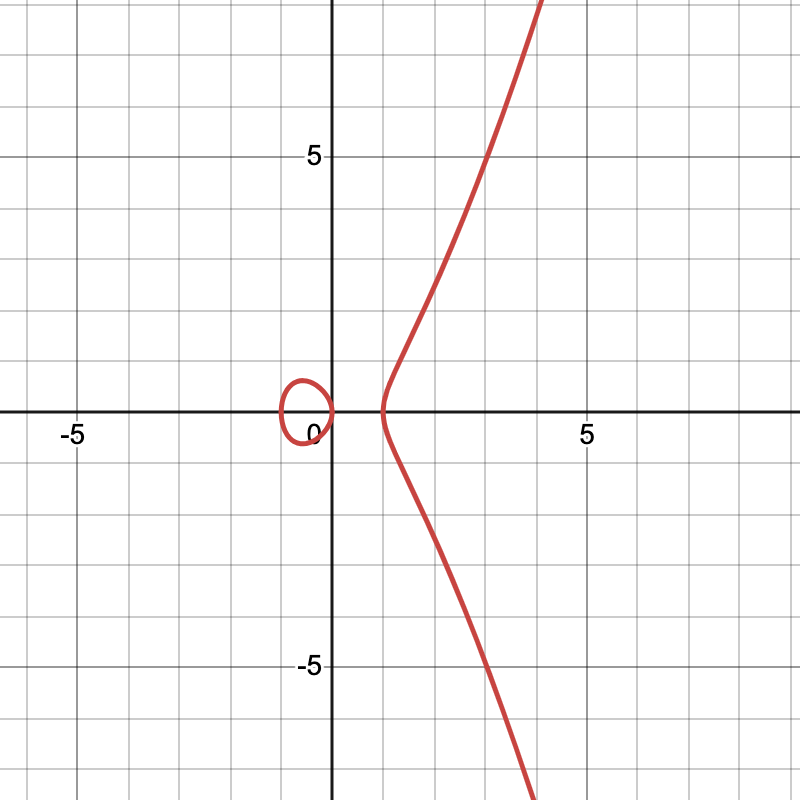
\includegraphics[scale = 0.2]{images/Varieties/desmos-graph2.png}
        \caption{$\V(y^2 - x(x+1)(x-1))$}
    \end{subfigure}
    \hfill
    \begin{subfigure}[b]{0.45\textwidth}
            \centering
            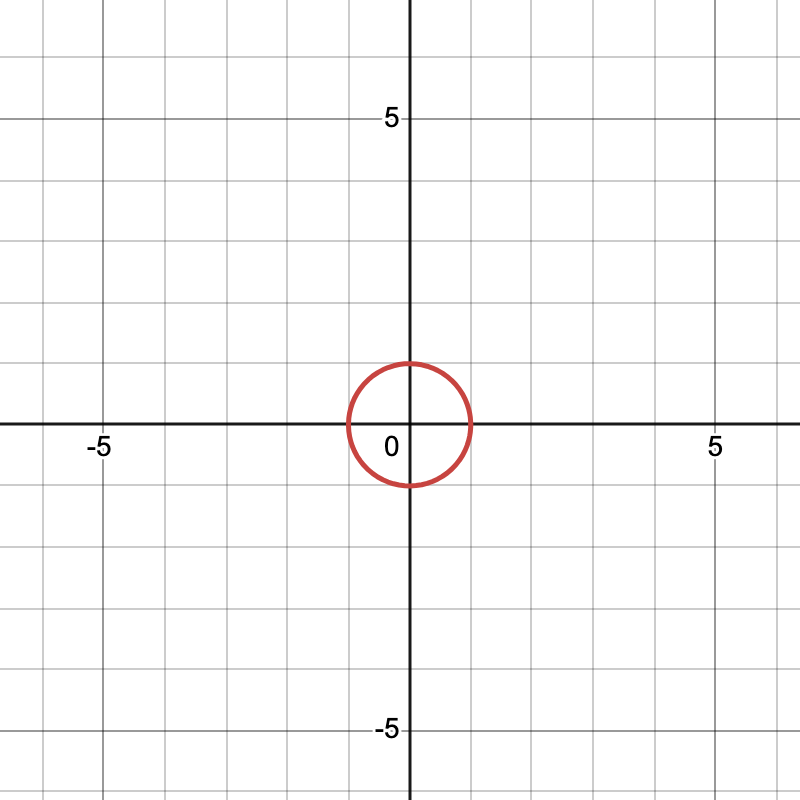
\includegraphics[scale = 0.2]{images/Varieties/desmos-graph.png}
            \caption{$\V(x^2 + y^2 - 1)$}
    \end{subfigure}
\caption{The vanishing locus of two separate polynomials plotted in $\R^2$}
\end{figure}

\subsection{Affine Varieties}
\subsection{Projective Varieties}
\subsection{Morphisms}
\subsection{Rational Maps}
\subsection{Nonsingular Varieties}
\subsection{Nonsingular Curves}
\subsection{Intersections in Projective Space}

\section{Schemes}
\subsection{Sheaves}
\subsection{Schemes}
\subsection{First Properties of Schemes}
\subsection{Separated and Proper Morphisms}
\subsection{Sheaves of Modules}
\subsection{Divisors}
\subsection{Projective Morphisms}
\subsection{Differentials}
\subsection{Formal Schemes}

\section{Cohomology}
\subsection{Derived Functors}
\subsection{Cohomology of Sheaves}
\subsection{Cohomology of a Noetherian Affine Scheme}
\subsection{Cech Cohomology}
\subsection{The Cohomology of Projective Space}
\subsection{Ext Groups and Sheaves}
\subsection{The Serre Duality Theorem}
\subsection{Higher Direct Images of Sheaves}
\subsection{Flat Morphisms}
\subsection{Smooth Morphisms}
\subsection{The Theorem on Formal Functions}
\subsection{The Semicontinuity Theorem}

\section{Curves}
\subsection{Riemann-Roch Theorem}
\subsection{Hurwitz's Theorem}
\subsection{Embeddings in Projective Space}
\subsection{Elliptic Curves}
\subsection{The Canonical Embedding}
\subsection{Classification of Curves in $\Proj^3$}

\section{Surfaces}
\subsection{Geometry on a Surface}
\subsection{Ruled Surfaces}
\subsection{Monoidal Transformations}
\subsection{The Cubic Surface in $\Proj^n$}\
\subsection{Birational Transformations}
\subsection{Classification of Surfaces}